\chapter[Prefixing-Based Method for Multiple Repetition Error Correction]{Prefixing-Based Method for  Multiple Repetition Error Correction}\label{prefixing}

 In this
chapter we propose a general prefixing method which injectively
transforms a given collection $C$ of binary strings of length $n$
into another collection of binary strings $D_C$ of equal length,
such that the collection $D_C$ is guaranteed to be immune to the
prescribed number of repetition errors. The proposed method is
inspired by the number-theoretic construction developed in the
previous chapter. It takes an element $\mathbf{c}$ of $C$ and
produces a string $\mathbf{t_c} =[\mathbf{p_c} \mathbf{c}]$,
$\mathbf{t_c} \in D_C$, that is, the prefix $\mathbf{p_c}$ is
prepended to $\mathbf{c}$ to produce $\mathbf{t_c}$. In the proposed
method, the set $D_C$ has the property that the length of the prefix
$\mathbf{p_c}$ is $O(\log(n))$. Thus, if the set $C$ is used for
transmission, the proposed method provides increased immunity to
repetition errors with asymptotically vanishing loss in the rate. We
also provide a message passing decoding algorithm suitable for
channels with both repetitions and additive errors whose complexity
is the same as of the traditional message passing decoding algorithm
designed to correct additive errors only.

 We start with some auxiliary
results. %%%%%%%%%% with draft 10/21/07

\section{Auxiliary results}\label{aux2} Consider a prime number $P$
with the property that $lcm(2,3,..r) | (P-1)$ for a given positive
integer $r$. Since each $i$, $1 \leq i \leq r$, satisfies $i|(P-1)$,
it follows that in the residue set $\mod P$, there are
$\frac{P-1}{i}$ elements that are $i$th power residues, each having
$i$ distinct roots (an $i$th power residue $x$ satisfies $y^i \equiv
x \mod P$ for some $y$), \cite{apostol}. For convenience, let $G =
\lfloor \log_2(P) \rfloor$.

For each $i$, $1 \leq i \leq r$, we will construct a specific subset
$V_i$ of the $i$th power residues $\mod P$ such that all other
residues can be expressed as a sum of a subset  of elements of
$V_i$, and such that each $V_i$ has size that is logarithmic in $P$.
The set of the $i$th roots of the elements of the set $V_i$ will be
denoted $F_i$. Thus, $F_i$ will also have size logarithmic in $P$.
The elements of $M =\bigcup_{i=1}^r F_i \cup \{0\}$ (the sets $F_i$
will be made disjoint) will be reserved for the weightings $f_i$ of
the bins of zeros of the prefix string $\mathbf{p_s}$ in the
transformed domain (see the construction ~\eqref{exten2}). Note that
$M$ also has size that is logarithmic in $P$, and since each bin in
the prefix will have at most one zero, the length of the prefix is
also logarithmic in $P$. The sets $V_i$ will serve to satisfy the
$i$th congruency constraint of the type given in~\eqref{exten2} for
the string $\mathbf{t_s}$ in the transformed domain, as further
explained below.

In the remainder of this section we will first show how to construct
sets $V_i$, and then we will provide the proof that it is possible
to construct sets $V_i$ with all distinct elements as well as  sets
$F_i$ (from sets $V_i$) that have distinct elements and are non
intersecting, for the prime $P$ large enough. We will also provide a
proof that for a given integer $n$, for $n$ large enough, there
exists a prime $P$ for which we can construct non intersecting sets
$F_i$ containing distinct elements, where the prime $P$ lies in an
interval that linearly depends on $n$.

Combined with the encoding method described in the next section we
will therefore have constructed a prefix whose length is logarithmic
in $n$ such that the overall string (which is a concatenation of the
prefix and original string) in the transformed domain satisfies
equations of congruential type given in~\eqref{exten2}, for which we
have already proved in the previous chapter are sufficient for the
immunity to $r$ repetition errors.



We now provide some auxiliary results. Let $[x]_P$ indicate the
residue mod $P$ congruent to $x$ .

\begin{lemma}\label{generates} For an integer $P$, each residue $v$ mod $P$ can be expressed as a
sum of a subset of elements of the set
$T_{z,P}=\{[z]_P,[2z]_P,[2^2z]_P,...,[2^{G}z]_P\}$ where $G=\lfloor
\log_2 P \rfloor $, $z$ is an arbitrary non zero residue mod $P$.
\end{lemma}

\noindent \textit{Proof:} Observe that
$T_{1,P}=\{1,2,2^2,...,2^{G}\}$. We first show that each residue $v$
mod $P$ can be expressed as a sum of a subset of elements of the set
$T_{1,P}$. Note that each residue $i$, $0 \leq i \leq 2^G-1$ (mod
$P$) can be expressed as a sum of a subset, call this subset $Q_i$,
of the set $\{1,2,2^2,...,2^{G-1}\}$. Here $Q_0$ is the empty set.
Adding $2^G$ to the sum of each $Q_i$, for $0 \leq i \leq 2^G-1$,
modulo $P$ generates the remaining residues $\{2^G, 2^G+1,...,P-1
\}$. As a result every residue mod $P$ can be expressed as a sum of
a subset of $T_{1,P}=\{1,2,2^2,...,2^{G}\}$.

Suppose there exists an element $v$ which cannot be expressed as a
sum of a subset of elements of $T_{z,P}$, for $z>1$, that is $v \neq
\sum_{i=0}^G \epsilon_i z 2^i \mod P$, for all choices of
$\{\epsilon_0,...,\epsilon_G\}$, $\epsilon_i \in \{0,1\}$. Let
$z^{-1}$ be the inverse element of $z$ under multiplication mod $P$.
Then the residue $v' = vz^{-1} \neq \sum_{i=0}^G \epsilon_i 2^i \mod
P$, for all choices of $\{\epsilon_0,...,\epsilon_G\}$, $\epsilon_i
\in \{0,1\}$, which contradicts the result from the previous
paragraph.\hfill$\blacksquare$




For a prime number $P$ for which $i|P-1$, and $i<P-1$, let $Q_i(P)$
be the set of distinct $i$th power residues mod $P$, let $N_i(P)$ be
the set of distinct $i$th power non residues mod $P$. We also state
the following convenient result.
\begin{lemma}\label{sums1}
For a prime $P$ such that $i | (P-1)$, each residue $n \mod P$ can
be expressed as a sum of two distinct elements of $Q_i(P)$ in at
least $P/(2i^2)-\sqrt{P}/2-3$ ways.
\end{lemma}
\noindent \textit{Proof:} The result follows from Theorem II in
\cite{huavan:49} which states that over $GF(P)$ the equation
\begin{equation}\label{hua} x^i+y^i=a
\end{equation} where $x,y,a \in GF(P)$ and nonzero and $0 < i <P-1 $
has at least
\begin{equation}\label{huasol}\frac{(P-1)^2}{P}-P^{-1/2}\left(1+(i-1)P^{1/2}\right)^2\end{equation}
solutions. Rearrange the terms in \eqref{huasol} to conclude that
\eqref{hua} has at least \begin{equation}\label{huasol1}
P-(i-1)^2\sqrt{P}-2(i-1)-2+\frac{1}{P}-\frac{1}{\sqrt{P}}
\end{equation} solutions. Noting that $i$ distinct values of $x$ result
in the same $x^i$, accounting for the symmetry of $x$ and $y$, and
omitting the case $x^i=y^i$ we obtain a lower bound on the number of
ways a residue can be expressed as a sum of two distinct $i$th power
residues to be $P/(2i^2)-\sqrt{P}/2-3$. \hfill$\blacksquare$

Equations of the type in (\ref{hua}) were also studied by Weil
\cite{weil:49}.



\comment{By Lemma~\ref{sums1}, for a prime $P$ it is sufficient that
$P/(2i^2)-\sqrt{P}/2-3>0$ for a nonzero residue $\mod P$ to be
expressed as a sum of two distinct $i$th power residues. In the
subsequent analysis we thus consider a prime number $P$ such that
$lcm(2,3,\dots,s)|(P-1)$ for the given positive integer $s$ and such
that $P>s^2(\sqrt{P}-6)$ (the condition  $P>s^2(\sqrt{P}-6)$
subsumes all conditions $P>i^2(\sqrt{P}-6)$ for $1 \leq i \leq s$).}

We now continue with the introduction of some convenient notation.
For $x_{i,1}$ an $i$th power residue define the set
$A_{i,1}(x_{i,1})$ to be
\begin{eqnarray}\label{azi1}A_{i,1}(x_{i,1})=\{[2^{ik}x_{i,1}]_P | 0 \leq k \leq
\lfloor\frac{G}{i} \rfloor \}~.\end{eqnarray} Let $x_{i,2}$ and
$x_{i,3}$ be distinct $i$th power residues such that
$x_{i,2}+x_{i,3} \equiv 2x_{i,1} \mod P$. %(possible by
%Lemma~\ref{sums1} since $P>i^2(\sqrt{P}-6)$).
These two power residues generate sets $A_{i,2}(x_{i,2})$ and
$A_{i,3}(x_{i,3})$ where
\begin{eqnarray}\label{azi2} A_{i,2}(x_{i,2}) =\{ [2^{ik}x_{i,2}]_P| 0 \leq k \leq \lfloor
\frac{G-1}{i} \rfloor \} \text{ and }\\
\label{azi3}A_{i,3}(x_{i,3}) =\{ [2^{ik}x_{i,3}]_P| 0 \leq k \leq
\lfloor \frac{G-1}{i} \rfloor \}~.\end{eqnarray}

Likewise, for each $2^lx_{i,1}$ for $1 \leq l \leq i-1$ let
$x_{i,2l}$ and $x_{i,2l+1}$ be distinct $i$th power residues such
that
$x_{i,2l} + x_{i,2l+1} \equiv 2^lx_{i,1} \mod P$. %(possible by
%Lemma~\ref{sums1}).
These residues generate sets $A_{i,2l}(x_{i,2l})$ and
$A_{i,2l+1}(x_{i,2l+1})$ where
\begin{eqnarray}\label{azi2l}
A_{i,2l}(x_{i,2l}) =\{ [2^{ik}x_{i,2l}]_P| 0 \leq k \leq \lfloor
\frac{G-l}{i} \rfloor \} \text{ and }\\
\label{azi2la}A_{i,2l+1}(x_{i,2l+1}) =\{ [2^{ik}x_{i,2l+1}]_P| 0
\leq k \leq \lfloor \frac{G-l}{i} \rfloor \}.\end{eqnarray}

By introducing sets $A_{i,j}(x_{i,j})$ we have effectively
decomposed all residues of the type $[2^{ik+l}x_{i,1}]_P$, $0 \leq
ik+l \leq G$, $1 \leq l \leq i-1$, for which $i$ is not a divisor of
$l$ into a sum of two $i$th power residues, namely
$[2^{ik}x_{i,2l}]_P$ and $[2^{ik}x_{i,2l+1}]_P$. For each set
$A_{i,j}(x_{i,j})$, $1 \leq j \leq 2i-1$, we let $B_{i,j}(x_{i,j})$
be the set of all $i$th power roots of elements of
$A_{i,j}(x_{i,j})$,
\begin{eqnarray}\label{bzi2l}
B_{i,j}(x_{i,j}) =\{ [2^{k}y_{i,j}^{(t)}]_P| (y_{i,j}^{(t)})^i
\equiv x_{i,j} \mod P, 1 \leq t \leq i, 0 \leq k \leq \lfloor
\frac{G-\lfloor \frac{j}{2} \rfloor}{i} \rfloor \}~.
\end{eqnarray}
First note that all elements in $A_{i,j}(x_{i,j})$ are $i$th power
residues by construction. Moreover, they are all distinct since
$2^{ij_1} \neq 2^{ij_2} \mod P$ for $1 \leq j_1,j_2 \leq \lfloor
\frac{G-\lfloor\frac{j}{2} \rfloor}{i} \rfloor$ for $j_1\neq j_2$
implies $x_{i,j}2^{ij_1} \neq x_{i,j}2^{ij_2} \mod P$. Thus,
$|A_{ij}(x_{i,j})|=\lfloor \frac{G-\lfloor \frac{j}{2}\rfloor}{i}
\rfloor+1$ and since the $i$th power roots of distinct $i$th power
residues are themselves distinct, $|B_{ij}(x_{i,j})|=i\left(\lfloor
\frac{G-\lfloor \frac{j}{2}\rfloor}{i} \rfloor+1\right)$.

\begin{lemma}\label{generates1} Suppose $P$ is a prime number such that $i|(P-1)$.
Let $x_{i,1}$ be an $i$th power residue. Suppose $x_{i,j}$ for $2
\leq j \leq 2i-1$ are $i$th power residues such that $2^{k}x_{i,1}
\equiv x_{i,2k}+x_{i,2k+1} \mod P$ for $1 \leq k \leq(i-1)$. Let
$A_{i,j}(x_{i,j}) =\{[2^{il}x_{i,j}]_P| 0 \leq l \leq \lfloor
\frac{G-\lfloor \frac{j}{2}\rfloor}{i}\rfloor\}$ for $1 \leq j \leq
2i-1$ and $G=\lfloor \log_2P \rfloor$. If the sets
$A_{i,j}(x_{i,j})$ are disjoint for $1 \leq j \leq 2i-1$, each
residue $n$ mod $P$ can be expressed as a sum of a subset of
elements of the set $L_{z,P}= \bigcup_{j=1}^{2i-1} A_{i,j}(x_{i,j})$
where $z$ denotes $x_{i,1}$.
\end{lemma}
\noindent \textit{Proof:} Follows immediately from
Lemma~\ref{generates} by observing that, with $z$ denoting
$x_{i,1}$, we have in fact decomposed elements $[2^{k}z]_P$ in the
set $T_{z,P}$ for $k$ not a multiple of $i$ into a sum of two
component elements such that all component elements are distinct
from one another and distinct from $[2^kz]_P$ for
$i|k$.\hfill$\blacksquare$

The following lemma proves that it is possible to construct subsets
$A_{ij}(x_{i,j})$, and subsets $B_{ij}(x_{i,j})$ from them, of the
set of residues $\mod P$ for $P$ prime that satisfies $lcm(2,3,...r)
| (P-1)$ for a given positive integer $r$, provided that $P$ is
large enough, such that for fixed $i$ the subsets $A_{ij}(x_{i,j})$
are disjoint, and such that \emph{all} subsets $B_{ij}(x_{i,j})$ for
$1 \leq i \leq r$, $1 \leq j \leq 2i-1$ are also disjoint. Let
$W_i(n)$ denote the number of ways any residue $n\mod P$ can be
expressed as a sum of two distinct non zero $i$th power residues
$\mod P$. A universal lower bound on $W_i(n)$ that holds for all
residues $n$ was given in Lemma~\ref{sums1}, and we will refer to it
as $W_i$.
\begin{lemma}\label{lemmaw} For a given integer $r$, suppose a prime number $P$ satisfies $lcm(2,3,...r) |
(P-1)$. Let $G =\lfloor \log_2{P}\rfloor$. If $P-1 >
(G+r)(G+r-1)(r-1)^2$ and $W_i
> 2i(G+i)(G+i-1)$, for each $i$ in the range $2 \leq i \leq
r$, there exist subsets $A_{ij}(x_{i,j})$ of the type given
in~\eqref{azi2l} and~\eqref{azi2la} and $B_{ij}(x_{i,j})$ of the
type given in~\eqref{bzi2l}
 such that for fixed $i$ subsets $A_{ij}(x_{i,j})$ for $1 \leq j \leq 2i-1$ are disjoint, and
for $1 \leq i \leq r$, $1 \leq j \leq 2i-1$ all subsets
$B_{ij}(x_{i,j})$ are disjoint.
\end{lemma}
\noindent \textit{Proof:} We inductively build the sets
$A_{ij}(x_{i,j})$ and $B_{ij}(x_{i,j})$ for $1 \leq i \leq r$ and $1
\leq j \leq 2i-1$, starting with the level $i=1$. We then increment
$i$ by one to reach the next collection of sets $A_{ij}(x_{i,j})$
and $B_{ij}(x_{i,j})$ while making sure the sets $B_{ij}(x_{i,j})$
at the current level are disjoint from one another and with all
previously constructed sets at lower levels.

Consider $i=1$. Let $x_{1,1}$ be an arbitrary residue$~\mod P$, and
let
\[A_{1,1}(x_{1,1})=\{[2^{k}x_{1,1}]_P | 0 \leq k \leq G \}.\] Let $z_1=x_{1,1}$ and $y_{1,1}^{(1)}=x_{1,1}$. Here
$B_{1,1}(z_1)$ is simply $A_{1,1}(x_{1,1})$ for $i=1$. All elements
in $B_{1,1}(z_{1})$ are distinct and $|B_{1,1}(z_{1})| =(G+1)$. If
$r=1$, we are done, as we did not even appeal to the condition on
the lower bound on $P-1$ (it is simply $P-1>0$).

If $r \geq 2$, let us consider $i=2$. Consider quadratic residues
$x_{2,1}$, $x_{2,2}$ and $x_{2,3}$. Let  their respective distinct
quadratic roots be $y_{2,1}^{(1)}$, $y_{2,1}^{(2)}$ (so that
$(y_{2,1}^{(1)})^2 \equiv (y_{2,1}^{(2)})^2 \equiv x_{2,1} \mod P$),
$y_{2,2}^{(1)}$, $y_{2,2}^{(2)}$ (so that $(y_{2,2}^{(1)})^2 \equiv
(y_{2,2}^{(2)})^2 \equiv x_{2,2} \mod P$) and $y_{2,3}^{(1)}$,
$y_{2,3}^{(2)}$ (so that $(y_{2,3}^{(1)})^2 \equiv (y_{2,3}^{(2)})^2
\equiv x_{2,3} \mod P$). These quadratic residues give rise to sets
\begin{eqnarray}
A_{2,1}(x_{2,1})&=&\{ [2^{2k}x_{2,1}]_P | 0 \leq k \leq \lfloor
\frac{G}{2} \rfloor\},\\ A_{2,2}(x_{2,2})&=& \{ [2^{2k}x_{2,2}]_P |
0
\leq k \leq \lfloor \frac{G-1}{2} \rfloor\} \text{ and},\\
A_{2,3}(x_{2,3})&=& \{ [2^{2k}x_{2,3}]_P | 0 \leq k \leq \lfloor
\frac{G-1}{2} \rfloor\}~.
\end{eqnarray}
Quadratic roots of elements of sets $A_{2,1}(x_{2,1})$,
$A_{2,2}(x_{2,2})$ and $A_{2,3}(x_{2,3})$ give rise to sets
$B_{2,1}(x_{2,1})$, $B_{2,2}(x_{2,2})$ and $B_{2,3}(x_{2,3})$,
\begin{eqnarray}
B_{2,1}(x_{2,1})&=&\{[2^ky_{2,1}^{(t)}]_P | 1 \leq t \leq 2, 0 \leq
k
\leq \lfloor \frac{G}{2}\rfloor\},\\
B_{2,2}(x_{2,2})&=&\{[2^ky_{2,2}^{(t)}]_P | 1 \leq t \leq 2, 0 \leq
k
\leq \lfloor \frac{G-1}{2}\rfloor\}, \text{ and}\\
B_{2,3}(x_{2,3})&=&\{[2^ky_{2,3}^{(t)}]_P | 1 \leq t \leq 2, 0 \leq
k \leq \lfloor \frac{G-1}{2}\rfloor\}~.
\end{eqnarray}


Having fixed the set $B_{1,1}(x_{1,1})$ based on the earlier
selection of the residue $x_{1,1}$, we want to show that it is
possible to find quadratic residues $x_{2,1}$, $x_{2,2}$ and
$x_{2,3}$ such that $x_{2,2} + x_{2,3} \equiv 2x_{2,1} \mod P$ and
such that the resulting sets $B_{1,1}(x_1)$, $B_{2,1}(x_{2,1})$,
$B_{2,2}(x_{2,2})$ and $B_{2,3}(x_{2,3})$ are all disjoint.

In particular we require that $x_{2,1}$ is a quadratic residue$~\mod
P$ (there are $(P-1)/2$ quadratic residues) with the property that
the set $B_{2,1}(x_{2,1})$ is disjoint from $B_{1,1}(x_{1,1})$. That
is we require \[y_{2,1}^{(1)}2^k \neq y_{1,1}^{(1)} 2^l \mod P \]
and
\[y_{2,1}^{(2)}2^k \neq y_{1,1}^{(1)} 2^l \mod P \] for $0 \leq k \leq \lfloor
\frac{G}{2} \rfloor$ and $0 \leq l \leq G$. By squaring the
expressions, these two conditions can be combined into
\begin{equation}\label{x21}x_{2,1}2^{2k} \neq (y_{1,1}^{(1)})^2 2^{2l} \mod P \end{equation}for $0
\leq k \leq \lfloor \frac{G}{2} \rfloor$ and $0 \leq l \leq G$. For
the already chosen $y_{1,1}^{(1)}(=x_{1,1})$ at most $(G+1)(\lfloor
\frac{G}{2} \rfloor+1)$ candidate quadratic residues out of total
$(P-1)/2$ quadratic residues violate ~\eqref{x21}. Observe that the
function $(G+i)(G+i-1)(i-1)^2$ is strictly increasing for positive
$i$, $2 \leq i \leq r$, and thus the condition $P-1>
(G+r)(G+r-1)(r-1)^2$ in the statement of the Lemma implies
$P-1>(G+2)(G+1)$. Since $\frac{P-1}{2} > \frac{(G+1)(G+2)}{2} \geq
(G+1)(\lfloor \frac{G}{2} \rfloor+1)$, such $x_{2,1}$ exists.

Fix $x_{2,1}$ such that \eqref{x21} holds. Having chosen such
$x_{2,1}$, we now look for $x_{2,2}$ and $x_{2,3}$ as distinct
quadratic residues that satisfy $x_{2,2}+x_{2,3} \equiv 2x_{2,1}
\mod P$. We require that $B_{2,2}(x_{2,2})$ be disjoint from both
$B_{1,1}(x_{1,1})$ and $B_{2,1}(x_{2,1})$ (by construction, if
$B_{2,2}(x_{2,2})$ and $B_{2,1}(x_{2,1})$ are disjoint so are
$A_{2,2}(x_{2,2})$ and $A_{2,1}(x_{2,1})$) so that
\begin{equation}\label{eqx22pre}\begin{array}{ccc}
y_{2,2}^{(1)}2^{k_3} \neq y_{1,1}^{(1)} 2^{k_1} \mod P, \\
y_{2,2}^{(2)}2^{k_3} \neq y_{1,1}^{(1)} 2^{k_1} \mod P,  \\
y_{2,2}^{(1)}2^{k_3} \neq y_{2,1}^{(1)} 2^{k_2} \mod P, \\
y_{2,2}^{(2)}2^{k_3} \neq y_{2,1}^{(1)} 2^{k_2} \mod P,  \\
y_{2,2}^{(1)}2^{k_3} \neq y_{2,1}^{(2)} 2^{k_2} \mod P, \\
y_{2,2}^{(2)}2^{k_3} \neq y_{2,1}^{(2)} 2^{k_2} \mod P,
\end{array}\end{equation}
where $0 \leq k_1 \leq G$, $0 \leq k_2 \leq \lfloor \frac{G}{2}
\rfloor$ and $0 \leq k_3 \leq \lfloor\frac{G-1}{2} \rfloor$.

Alternatively, by squaring both sides in each expression in
\eqref{eqx22pre},
\begin{equation}\label{eqx22}\begin{array}{cccc}
x_{2,2}2^{2k_3} &\neq& (y_{1,1}^{(1)})^2 2^{2k_1} &\mod P, \\
x_{2,2}2^{2k_3} &\neq& x_{2,1} 2^{2k_2} &\mod P,
\end{array}\end{equation}
where $0 \leq k_1 \leq G$, $0 \leq k_2 \leq \lfloor \frac{G}{2}
\rfloor$ and $0 \leq k_3 \leq \lfloor\frac{G-1}{2} \rfloor$.

Likewise, we require that $B_{2,3}(x_{2,3})$ be disjoint from
$B_{1,1}(x_{1,1})$, $B_{2,1}(x_{2,1})$ and  $B_{2,2}(x_{2,2})$
(again, if $B_{2,3}(x_{2,3})$ is disjoint from $B_{2,2}(x_{2,2})$
and $B_{2,1}(x_{2,1})$, then $A_{2,3}(x_{2,3})$ is disjoint from
$A_{2,2}(x_{2,2})$ and $A_{2,1}(x_{2,1})$) so that
\begin{equation}\label{eqx23}\begin{array}{cccc}
x_{2,3}2^{2k_4} &\neq& (y_{1,1}^{(1)})^2 2^{2k_1} &\mod P, \\
x_{2,3}2^{2k_4} &\neq& x_{2,1} 2^{2k_2} &\mod P, \\
x_{2,3}2^{2k_4} &\neq& x_{2,2} 2^{2k_3} &\mod P, \\
\end{array}\end{equation}
where $0 \leq k_1 \leq G$, $0 \leq k_2 \leq \lfloor \frac{G}{2}
\rfloor$, $0 \leq k_3 \leq \lfloor\frac{G-1}{2} \rfloor$ and $0 \leq
k_4 \leq \lfloor\frac{G-1}{2} \rfloor$. For the already chosen
values of $x_{2,1}$ and $y_{1,1}$ at most $N_2= 2\left[
\left(\lfloor \frac{G}{2} \rfloor +1 \right)\left(\lfloor
\frac{G-1}{2} \rfloor +1 \right)+ \left( G+1 \right)\left(\lfloor
\frac{G-1}{2} \rfloor +1 \right)\right]+\left( \lfloor \frac{G-1}{2}
\rfloor +1 \right)^2  $ choices for $x_{2,2}$ and $x_{2,3}$
violate~\eqref{eqx22} and ~\eqref{eqx23}.

We thus require that $W_2$ be strictly larger than $N_2$. Dropping
floor operations it is sufficient that $W_2 > \frac{(G+1)(G+2)}{2} +
\frac{5(G+1)^2}{4}$. Further  simplification yields that
\begin{equation}
W_2 > \frac{7(G+1)(G+2)}{4}
\end{equation}
is sufficient to ensure that there exist $x_{2,2}$, $x_{2,3}$ that
make the respective sets disjoint. Note that this last condition
follows from the requirement in the statement of the Lemma for
$i=2$, namely that $W_2 > 4(G+1)(G+2)$. If $r=2$ we are done, else
we consider $i=3$. Before considering general level $i$ let us
present the $i=3$ case.

For $i=3$ we seek distinct cubic residues $x_{3,1}$, $x_{3,2}$,
$x_{3,3}$, $x_{3,4}$ and $x_{3,5}$ with the property that $x_{3,2}+
x_{3,3} \equiv 2x_{3,1} \mod P$ and $x_{3,4}+ x_{3,5} \equiv
2^2x_{3,1} \mod P$, and such that the respective sets
$B_{3,j}(x_{3,j})$ for $1 \leq j \leq 5$ generated from the cubic
roots of these residues are disjoint and are disjoint from
previously constructed sets $B_{1,1}(x_{1,1})$, $B_{2,1}(x_{2,1})$,
$B_{2,2}(x_{2,2})$ and $B_{2,3}(x_{2,3})$.


We start with $x_{3,1}$ a cubic residue$~\mod P$ (there are
$(P-1)/3$ cubic residues) with the property that the set
$B_{3,1}(x_{3,1})$ is disjoint from each of $B_{1,1}(x_{1,1})$,
$B_{2,1}(x_{2,1})$, $B_{2,2}(x_{2,2})$ and $B_{2,3}(x_{2,3})$. That
is, after raising the elements of these sets to the third power, we
require
\begin{equation}\label{eqx31}\begin{array}{cccc}
x_{3,1}2^{3k_4} &\neq& (y_{1,1}^{(1)})^3 2^{3k_1} &\mod P, \\
x_{3,1}2^{3k_4} &\neq& (y_{2,1}^{(1)})^3 2^{3k_2} &\mod P, \\
x_{3,1}2^{3k_4} &\neq& (y_{2,1}^{(2)})^3 2^{3k_2} &\mod P, \\
x_{3,1}2^{3k_4} &\neq& (y_{2,2}^{(1)})^3 2^{3k_3} &\mod P, \\
x_{3,1}2^{3k_4} &\neq& (y_{2,2}^{(2)})^3 2^{3k_3} &\mod P, \\
x_{3,1}2^{3k_4} &\neq& (y_{2,3}^{(1)})^3 2^{3k_3} &\mod P, \\
x_{3,1}2^{3k_4} &\neq& (y_{2,3}^{(2)})^3 2^{3k_3} &\mod P, \\
\end{array}\end{equation}
where $0 \leq k_1 \leq G$, $0 \leq k_2 \leq \lfloor \frac{G}{2}
\rfloor$, $0 \leq k_3 \leq \lfloor\frac{G-1}{2} \rfloor$ and $0 \leq
k_4 \leq \lfloor\frac{G}{3} \rfloor$.

For the already chosen values of $x_{1,1}$ through $x_{2,3}$, which
in turn determine $y_{1,1}^{(1)}$ through $y_{2,3}^{(2)}$, the
condition in~\eqref{eqx31} prevents $N_3= \left(\lfloor \frac{G}{3}
\rfloor +1 \right)\left[ (G+1)+2\left(\lfloor \frac{G}{2} \rfloor +1
\right) +4\left(\lfloor \frac{G-1}{2} \rfloor +1 \right)\right]$
choices for $x_{3,1}$. Since there are $\frac{P-1}{3}$ cubic
residues, after simplifying and upper bounding the expression for
$N_3$, it follows that it is sufficient that $\frac{P-1}{3}$ be
strictly larger than $\frac{4(G+2)(G+3)}{3}$. Note that this
condition is implied by the requirement that $P-1>
(r-1)^2(G+r)(G+r-1)$ (again, since the function
$(i-1)^2(G+i)(G+i-1)$ is strictly increasing for positive $i$).

Fix $x_{3,1}$ such that \eqref{eqx31} holds. Having chosen such
$x_{3,1}$, we now look for distinct $x_{3,2}$, $x_{3,3}$, $x_{3,4}$,
$x_{3,5}$ cubic residues that satisfy $x_{3,2}+x_{3,3} \equiv
2x_{3,1} \mod P$ and $x_{3,4}+x_{3,5} \equiv 2^2x_{3,1} \mod P$ that
make all sets $B_{i,j}(x_{i,j})$, $1 \leq i \leq 3$, $1 \leq j \leq
2i-1$ disjoint.

In order that residue $x_{3,2}$ generates set $B_{3,2}(x_{3,2})$
with the property that $B_{3,2}(x_{3,2})$ is disjoint from each of
$B_{1,1}(x_{1,1})$, $B_{2,1}(x_{2,1})$, $B_{2,2}(x_{2,2})$,
$B_{2,3}(x_{2,3})$ and $B_{3,1}(x_{3,1})$, we require that their
respective elements raised to the third power be distinct,
\begin{equation}\label{eqx32}\begin{array}{cccc}
x_{3,2}2^{3k_5} &\neq& (y_{1,1}^{(1)})^3 2^{3k_1} &\mod P, \\
x_{3,2}2^{3k_5} &\neq& (y_{2,1}^{(1)})^3 2^{3k_2} &\mod P, \\
x_{3,2}2^{3k_5} &\neq& (y_{2,1}^{(2)})^3 2^{3k_2} &\mod P, \\
x_{3,2}2^{3k_5} &\neq& (y_{2,2}^{(1)})^3 2^{3k_3} &\mod P, \\
x_{3,2}2^{3k_5} &\neq& (y_{2,2}^{(2)})^3 2^{3k_3} &\mod P, \\
x_{3,2}2^{3k_5} &\neq& (y_{2,3}^{(1)})^3 2^{3k_3} &\mod P, \\
x_{3,2}2^{3k_5} &\neq& (y_{2,3}^{(2)})^3 2^{3k_3} &\mod P, \\
x_{3,2}2^{3k_5} &\neq& x_{3,1} 2^{3k_4} &\mod P,
\end{array}\end{equation}
where $0 \leq k_1 \leq G$, $0 \leq k_2 \leq \lfloor \frac{G}{2}
\rfloor$, $0 \leq k_3 \leq \lfloor\frac{G-1}{2} \rfloor$, $0 \leq
k_4 \leq \lfloor\frac{G}{3} \rfloor$ and $0 \leq k_5 \leq
\lfloor\frac{G-1}{3} \rfloor$.

Likewise, we require that $B_{3,3}(x_{3,3})$ be disjoint from all of
$B_{1,1}(x_{1,1})$, $B_{2,1}(x_{2,1})$, $B_{2,2}(x_{2,2})$,
$B_{2,3}(x_{2,3})$, $B_{3,1}(x_{3,1})$ and $B_{3,2}(x_{3,2})$, so
that
\begin{equation}\label{eqx33}\begin{array}{cccc}
x_{3,3}2^{3k_6} &\neq& (y_{1,1}^{(1)})^3 2^{3k_1} &\mod P, \\
x_{3,3}2^{3k_6} &\neq& (y_{2,1}^{(1)})^3 2^{3k_2} &\mod P, \\
x_{3,3}2^{3k_6} &\neq& (y_{2,1}^{(2)})^3 2^{3k_2} &\mod P, \\
x_{3,3}2^{3k_6} &\neq& (y_{2,2}^{(1)})^3 2^{3k_3} &\mod P, \\
x_{3,3}2^{3k_6} &\neq& (y_{2,2}^{(2)})^3 2^{3k_3} &\mod P, \\
x_{3,3}2^{3k_6} &\neq& (y_{2,3}^{(1)})^3 2^{3k_3} &\mod P, \\
x_{3,3}2^{3k_6} &\neq& (y_{2,3}^{(2)})^3 2^{3k_3} &\mod P, \\
x_{3,3}2^{3k_6} &\neq& x_{3,1} 2^{3k_4} &\mod P, \\
x_{3,3}2^{3k_6} &\neq& x_{3,2} 2^{3k_5} &\mod P,
\end{array}\end{equation}
where $0 \leq k_1 \leq G$, $0 \leq k_2 \leq \lfloor \frac{G}{2}
\rfloor$, $0 \leq k_3 \leq \lfloor\frac{G-1}{2} \rfloor$, $0 \leq
k_4 \leq \lfloor\frac{G}{3} \rfloor$, $0 \leq k_5 \leq
\lfloor\frac{G-1}{3} \rfloor$ and $0 \leq k_6 \leq
\lfloor\frac{G-1}{3} \rfloor$.

From~\eqref{eqx32} and~\eqref{eqx33} it follows that at most
\begin{equation}\label{w31}\begin{array}{lll} N_3'=&2 \left( \lfloor \frac{G-1}{3}\rfloor +1\right) \left[
(G+1)+2\left( \lfloor \frac{G}{2}\rfloor +1\right) +4\left( \lfloor
\frac{G-1}{2}\rfloor +1\right) + \left( \lfloor \frac{G}{3}\rfloor
+1\right)\right]+ \\{}&\left( \lfloor \frac{G-1}{3}\rfloor
+1\right)^2.
\end{array}\end{equation}
candidate pairs $(x_{3,2},x_{3,3})$ do not make the respective
$B_{i,j}(x_{i,j})$ sets disjoint. Since
\begin{equation}\label{w31a}\begin{array}{lll}
N_3'& \leq &2\left( \frac{G+2}{3} \right) \left[ (G+1)+2\left(
\frac{G+2}{2}\right) +4\left( \frac{G+1}{2}\right) + \left(
\frac{G+3}{3}\right)\right]+\left(  \frac{G+2}{3}
\right)^2\\
{}&<&2\left( \frac{G+2}{3} \right) \cdot
13\left(\frac{G+3}{3}\right)+\left( \frac{G+2}{3} \right)^2\\
{}&<&3(G+2)(G+3),
\end{array}\end{equation} it follows that it is sufficient that
\begin{equation}\label{w311}
W_3 > 3 (G+2)(G+3)~,
\end{equation}
where $W_3$ is the number of ways a residue $\mod P$ can be
expressed as a sum of two different cubic residues. Similarly, the
cubic residues $x_{3,4}$ and $x_{3,5}$ for which the respective
disjoint $B_{i,j}(x_{i,j})$ sets  exist, provided that
\begin{equation}\label{w31a}\begin{array}{lll} W_3
> 2 \left( \lfloor \frac{G-2}{3}\rfloor +1\right)\left[
(G+1)+2\left( \lfloor \frac{G}{2}\rfloor +1\right) +4\left( \lfloor
\frac{G-1}{2}\rfloor +1\right)  +\left( \lfloor \frac{G}{3}\rfloor
+1\right)+\right.\\\left.2\left( \lfloor \frac{G-1}{3}\rfloor
+1\right)\right]+ \left( \lfloor \frac{G-2}{3}\rfloor +1\right)^2.
\end{array}\end{equation}
 Some simplification of ~\eqref{w31a} yields
\begin{equation}\label{w312}
W_3 > \frac{31}{9} (G+2)(G+3)~,
\end{equation}
which subsumes the lower bound on $W_3$ given in ~\eqref{w311}. Note
that ~\eqref{w312} is implied by the condition in the statement of
the Lemma, namely $W_3 >6(G+2)(G+3)$.

We now inductively show the existence of the appropriate $i$th power
residues and their sets, assuming that we have successfully
identified power residues at lower levels for which all the sets
$B_{k,j}(x_{k,j})$ for $1 \leq k <i$, $1 \leq j \leq 2k-1$ are
disjoint.

Consider $x_{i,1}$ an $i$th power residue$~\mod P$ (there are
$(P-1)/i$ such  residues) with the property that the set
$B_{i,1}(x_{i,1})$ is disjoint from all of $B_{k,j}(x_{k,j})$ for $1
\leq k <i$, $1 \leq j \leq 2k-1$.

These  constraints on disjointness (an example of which is given
in~\eqref{x21} for $i=2$ and in ~\eqref{eqx31} for $i=3$) prevent no
more than $(\frac{G+i}{i})(\frac{G+k}{k})$ choices for $x_{i,1}$ for
each $y_{k,j}^{(t)}$ where $1 \leq k \leq i-1$, $1 \leq j \leq
2k-1$, and $1 \leq t \leq k$ (since $|B_{i,1}(x_{i,1})|=\lfloor
\frac{G}{i} \rfloor+1 \leq \frac{G+i}{i}$, and
$|B_{k,j}(x_{k,j})|=\lfloor \frac{G-\lfloor \frac{j}{2}\rfloor}{k}
\rfloor+1 \leq \frac{G+k}{k}$). Summing over all choices it follows
that at most
\begin{equation}\begin{array}{lll}{}& \left(\frac{G+i}{i}\right) \sum_{k=1}^{i-1}
(2k-1)k\left(\frac{G+k}{k}\right)\\\leq&
(G+i)\left(\frac{G+i-1}{i}\right) \sum_{k=1}^{i-1}
(2k-1)\\=&(G+i)\left(\frac{G+i-1}{i}\right)(i-1)^2
\end{array}\end{equation} $i$th power residues cannot be chosen for
$x_{i,1}$. Since there are $\frac{P-1}{i}$ $i$th power residues, we
thus require
\begin{equation}\label{preq}
P-1 > (G+i)(G+i-1)(i-1)^2
\end{equation}
for each level $i$. Note that since the expression on the right hand
side of the inequality ~\eqref{preq} is an increasing function of
positive $i$, each subsequent level poses a lower bound on $P$ that
subsumes all previous ones. It is thus sufficient to have $P-1
> (G+r)(G+r-1)(r-1)^2$, as given in the statement of the Lemma.

Consider $x_{i,2}$ and $x_{i,3}$ as distinct $i$th power
residues$~\mod P$ that satisfy $x_{i,2}+ x_{i,3} \equiv 2x_{i,1}
\mod P$ for a previously chosen $x_{i,1}$. We require that
 $x_{i,2}$ and $x_{i,3}$ give rise to sets $B_{i,2}(x_{i,2})$ and
$B_{i,3}(x_{i,3})$ that are disjoint and that are disjoint from each
of $B_{k,j}(x_{k,j})$ for $1\leq k < i$, $1\leq j \leq 2k-1$ and
with $B_{i,1}(x_{i,1})$. By construction, if the sets
$B_{i,1}(x_{i,1})$, $B_{i,2}(x_{i,2})$, and $B_{i,3}(x_{i,3})$ are
disjoint, then so are sets $A_{i,1}(x_{i,1})$, $A_{i,2}(x_{i,2})$,
and $A_{i,3}(x_{i,3})$. Constraints based on the previously
encountered $y_{j,k}^{(t)}$ for $1\leq k < i$, $1\leq j \leq 2k-1$,
$1 \leq t \leq k$ prevent at most $(\frac{G+i-1}{i})(\frac{G+j}{j})$
choices for each of $x_{i,2}$ and $x_{i,3}$, for each
$y_{j,k}^{(t)}$ (since $|B_{i,2}(x_{i,2})|=|B_{i,3}(x_{i,3})|=
\lfloor \frac{G-1}{i} \rfloor+1 \leq \frac{G+i-1}{i}$, and
$|B_{k,j}(x_{k,j})|=\lfloor \frac{G-\lfloor \frac{j}{2}\rfloor}{k}
\rfloor+1 \leq \frac{G+k}{k}$). Combined with the restriction based
on the disjointness with $B_{i,1}(x_{i,1})$ and the requirement that
$B_{i,2}(x_{i,2})$ and $B_{i,3}(x_{i,3})$ be nonintersecting, it
follows that
\begin{equation}\begin{array}{lll} W_i>
2\left(\frac{G+i-1}{i}\right) \left[\sum_{k=1}^{i-1}
(2k-1)k(\frac{G+k}{k})+\left( \frac{G+i}{i}\right)\right]+\left(
\frac{G+i-1}{i}\right)^2
\end{array}\end{equation}
is sufficient for the pair $(x_{i,2},x_{i,3})$ to exist.

Likewise, for  $x_{i,2l}$ and $x_{i,2l+1}$ to be distinct $i$th
power residues$~\mod P$ that satisfy $x_{i,2l}+ x_{i,2l+1} \equiv
2^lx_{i,1} \mod P$, that give rise to disjoint sets
$B_{i,2l}(x_{i,2l})$ and $B_{i,2l+1}(x_{i,2l+1})$ and that are also
disjoint from all previously constructed set $B_{k,j}(x_{k,j})$, we
require
\begin{equation}\label{eqwi}\begin{array}{lll} W_i>
2(\frac{G+i-1}{i}) \left[\sum_{k=1}^{i-1}
(2k-1)k(\frac{G+k}{k})+(2l-1)\left(
\frac{G+i}{i}\right)\right]+\left( \frac{G+i-1}{i}\right)^2
\end{array}\end{equation}
for the pair $(x_{i,2l},x_{i,2l+1})$ to exist. Since at each level
$i$ we construct $i-1$ pairs $x_{i,2l}$ and $x_{i,2l+1}$, and since
the right hand side of~\eqref{eqwi} is an increasing function of
$l$, it is sufficient to upper bound the expression in ~\eqref{eqwi}
for $l=i-1$,
\begin{equation}\label{eqwi}\begin{array}{lll} {}&W_i>
2(\frac{G+i-1}{i}) \left[\sum_{k=1}^{i-1}
(2k-1)k(\frac{G+k}{k})+(2i-3)\left(
\frac{G+i}{i}\right)\right]+\left( \frac{G+i-1}{i}\right)^2\\
\Leftarrow & W_i > 2(\frac{G+i-1}{i}) \left[
(i-1)^2(G+i)+\frac{2i-3}{i} (G+i)\right]+\left(
\frac{G+i-1}{i}\right)^2 \\\Leftarrow & W_i > (G+i)(G+i-1) \left(
\frac{2}{i}(i-1)^2+\frac{2}{i}\frac{2i-3}{i}+\frac{1}{i^2} \right)~.
\end{array}\end{equation}


Some simplification yields
\begin{equation}\begin{array}{lll} W_i>
(G+i)(G+i-1)\frac{2i^3-4i^2+6i-5}{i^2}
\end{array}\end{equation}
as a sufficient condition for the disjoint sets $B_{i,j}(x_{i,j})$
to exist that are also disjoint from all sets $B_{k,l}(x_{k,l})$ for
$k<i$.

Further simplifying the last inequality, it is sufficient that
\begin{equation}\begin{array}{lll} W_i>
2i(G+i)(G+i-1)
\end{array}\end{equation}
to make these sets disjoint. We have thus demonstrated that with the
appropriate lower bounds on $P$ and $W_i$'s, it is possible to
construct disjoint sets $B_{i,j}(x_{i,j})$.
 \hfill$\blacksquare$

Note that all residues$~\mod P$ can be expressed as a sum of a
subset of elements of $V_i \asn
\bigcup_{j=1}^{2i-1}A_{i,j}(x_{i,j})$ by Lemma~\ref{generates1} for
each $i$, $1\leq i \leq r$. Also note that $|V_i|$ scales as
$\log_2(P)$, since $|A_{i,j}(x_{i,j})|=\lfloor \frac{G-\lfloor
\frac{j}{2} \rfloor}{i}\rfloor+1$. For $F_i \asn
\bigcup_{j=1}^{2i-1}B_{ij}(x_{i,j})$,
 $|F_i|$ also scales as
$\log_2(P)$, since  $|B_{i,j}(x_{i,j})|=i\left(\lfloor
\frac{G-\lfloor \frac{j}{2} \rfloor}{i}\rfloor+1\right)$.




We now discuss how large prime $P$ needs to be so that the
conditions of Lemma~\ref{lemmaw} hold. Namely we require
\begin{equation}\label{ne1}
P-1> (r-1)^2(G+r)(G+r-1) \end{equation} and
\begin{equation}\label{ne2}W_i>2i(G+i)(G+i-1) \text{ for }2 \leq i \leq r~. \end{equation} Using
Lemma~\ref{sums1} it follows that it is sufficient that
\begin{equation}\label{condp}
P > 4r^3(G+r)(G+r-1)+r^2\sqrt{P}+6r^2~, \text{for } r \geq 2
\end{equation}
for  ~\eqref{ne2} to hold.  Moreover, if \eqref{condp} holds , it
implies \eqref{ne1}.(For $r=1$, the requirement is $P>1$). The
expression \eqref{condp} certainly holds as $P\rightarrow \infty$,
and for the finite values of $P$ we (loosely) have that
\begin{eqnarray*}
P>200 \text{ for } r=1, \\P>4\times 10^3 \text{ for } r=2,
\\P>2\times 10^4 \text{ for } r=3,\\ P>6\times 10^4 \text{ for }
r=4,\\P>2 \times 10^5 \text{ for } r=5.
\end{eqnarray*}

 For a given large enough integer $n$, we now show that
there exists a prime number $P$ that satisfies~\eqref{condp} (which
holds for $P$ large enough) and for which $lcm(2,3,...,r) | (P-1)$
such that $P$ lies in an interval that is linear in $n$. Since the
elements of $M \asn \bigcup_{i=1}^r F_i \cup \{0\}$ are to be
reserved for the indices of bins of zeros of the prefix in the
transformed domain we also require that $P-n > |M|$, since the total
number of bins of zeros to be used is at most $n$ (from the original
string) + $|M|$ (from the prefix), and each bin receives a distinct
index. Since $F_i= \cup_{j=1}^{2i-1} B_{i,j}(x_{i,j})$ and
$|B_{i,j}(x_{i,j})|$ =$i\left( \lfloor \frac{G-\lfloor
\frac{j}{2}\rfloor}{i}\rfloor+1\right)$, whereby $i\left(\frac
{G-i}{i}\right) \leq |B_{i,j}(x_{i,j})|\leq i
\left(\frac{G+i}{i}\right)$, it follows that
\begin{equation}\label{eqM} |M| \leq \sum_{i=1}^r (2i-1)(G+i) +1
\leq (G+r) \sum_{i=1}^r (2i-1) =r^2(G+r)+1\end{equation} and
\begin{equation}\label{eqM2} |M| \geq \sum_{i=1}^r (2i-1)(G-i) +1
\geq  (G-r) \sum_{i=1}^r (2i-1) =r^2(G-r)+1\end{equation}


Equation \eqref{eqM} yields a sufficient requirement on how large
$P$ needs to be
\begin{equation}\label{condpn}P>n+r^2(\log_2(P)+r)+1~.
\end{equation}

For given integers $n$ and $r$ ($n$ is typically large and $r$ is
small), we essentially need to show that there exists a prime $P$
for which $k \asn lcm(2,3,...,r) | (P-1)$ and $P \in (c_1n,c_2n)$
(here $c_1$ and $c_2$ are positive numbers that do not depend on
$n$) and such that $P$ satisfies~\eqref{condp} and~\eqref{condpn}.

For the asymptotic regime as $n \rightarrow \infty$ we recall the
prime number theorem for arithmetic progressions \cite{sopro} which
states that
\begin{equation}
\pi(n,k,1) \sim \frac{1}{\phi(k)} \frac{n}{\log(n)}~,
\end{equation}
where $\pi(n,k,1)$ denotes the number of primes $\leq n$ that are
congruent to $1 \mod k$, and $\phi(k)$ is the Euler function and
represents the number of integers $\leq k$ that are relatively prime
with $k$. As $n \rightarrow \infty$, we may let $c_1 \asn 2$ and
$c_2 \asn 4$, so that
\begin{equation}
\frac{\pi(4n,k,1)}{\pi(2n,k,1)} \sim 2~,
\end{equation}
and thus there exists a prime $P$, $k | (P-1)$ in an interval that
is linear in $n$. Clearly, as $n \rightarrow \infty$, such $P$ also
satisfies ~\eqref{condp} and~\eqref{condpn}.



For finite (but possibly very large) values of $n$ and certain small
$r$ we appeal to results by Ramare and Rumely \cite{rrumely}. The
number-theoretic function $\theta(x;k,l)$ is usually defined as
\[\theta(x;k,l)=\sum_{p \text{ prime }, p \equiv l\mod k, p
\leq x} \ln p~.\]

To show that there exists a prime $P$ in the interval $(c_1n,c_2n)$
for which $k=lcm(2,3,...,r) | (P-1)$  it is sufficient to have
\begin{equation} \label{thetas}\theta(c_2n;k,1)> \theta(c_1n;k,1)~,\end{equation}
where $k=lcm(2,3,...,r)$.

Theorem 2 in \cite{rrumely} states that $|\theta(x;k,1)
-\frac{x}{\phi(k)}| \leq 2.072 \sqrt{x}$ for all $x \leq 10 ^{10}$
for $k$ given in Table I of \cite{rrumely}. For larger $x$, Theorem
1 in \cite{rrumely}, provides the bounds of the type
\begin{equation}
(1-\varepsilon)\frac{x}{\phi(k)} \leq \theta(x;k,1) \leq
(1+\varepsilon)\frac{x}{\phi(k)}~,
\end{equation}
for $k$ given in Table I of \cite{rrumely}, and $\varepsilon$ also
given in Table I of \cite{rrumely} for various $x$. Here $\phi(k)$
is the Euler function and denotes the number of integers $\leq k$
that are relatively prime with $k$.


For $c_2n < 10^{10}$, using \[\theta(c_1n;k,1) <
\frac{c_1n}{\phi(k)}+2.072\sqrt{c_1n}
\]
and \[\theta(c_2n;k,1) > \frac{c_2n}{\phi(k)}-2.072\sqrt{c_2n},
\]it is thus sufficient to have
\begin{equation}\label{cond1}
2.072\phi(k) < \sqrt{n}(\sqrt{c_2}-\sqrt{c_1})~,
\end{equation}
for $\theta(c_2n;k,1)> \theta(c_1n;k,1)$ to hold.


For $c_1n>10^{10}$ using \[\theta(c_1n;k,1) < (1+\varepsilon)
\frac{c_1n}{\phi(k)}
\]
and \[\theta(c_2n;k,1) > (1-\varepsilon)\frac{c_2n}{\phi(k)},
\] after some simplification, it is sufficient to have
\begin{equation}\label{cond1a}
(1+\varepsilon)c_1 < (1-\varepsilon)c_2~,
\end{equation}
for $\theta(c_2n;k,1)> \theta(c_1n;k,1)$ to hold.

 Expressing $P \in (c_1n,c_2n)$ in terms of $c_1n$ and $c_2n$, it is
sufficient that
\begin{equation}\label{cond2}
(c_1-1)n > r^2(\log_2n+\log_2c_2+r)+1
\end{equation}
for~\eqref{condpn} to hold. Likewise, for $r \geq 2$, it is
sufficient that
\begin{equation}\label{cond3}
c_1n>4r^3(\log_2n+\log_2c_2+r)(\log_2n+\log_2c_2+r-1)+r^2(6+\sqrt{c_2n})
\end{equation}
for~\eqref{condp} to hold.

%For $c_1n>10^{10}$ the condition~\eqref{cond1} is replaced by XXX
%(see Theorem 1 in \cite{rrumely}).



Parameters $c_1$ and $c_2$ can be chosen as a function of $r$ to
make~\eqref{cond1} (or~\eqref{cond1a}), ~\eqref{cond2} and
~\eqref{cond3} hold. We consider now some suitable choices for $c_1$
and $c_2$ for small values of $r$ and some finite $n$.
\begin{itemize}
\item $r=1$: The condition ~\eqref{cond2} reduces to $(c_1-1)n >
\log_2(n)+\log_2(c_2)+2$. For $c_2n < 10^{10}$, the condition
~\eqref{cond1} reduces to $\sqrt{n}(\sqrt{c_2}-\sqrt{c_1})> 2.072$.
We may let $c_2=4$ and $c_1=2$ for $12<n<10^{10}/4$ to ensure that
there exists a prime in the interval $(2n,4n)$ which satisfies
~\eqref{cond2}.

The condition ~\eqref{cond1a} applies to $c_1n>10^{10}$ so we may
let $c_1=4$
 for $n>10^{10}/4$. Since all $\varepsilon$ entries for $k=1$ in Table I of \cite{rrumely}
 are $\ll 1/9$, we may let $c_2=5$ to make the condition \eqref{cond2} hold .

 Since $|M| \leq (\lfloor\log_2P\rfloor+2)\leq (\log_2 n+\log_2 c_2+2)$ (from~\eqref{eqM}), and
$|M| \geq \lfloor \log_2P\rfloor\geq (\log_2 n+\log_2 c_1-2)+1$
(from~\eqref{eqM2})
 it
 follows that $(\log_2n) \leq |M| \leq (\log_2n+4 )$ for $12<n<10^{10}/4$ and $(\log_2 n+1) \leq |M| \leq (\log_2n+5 )$ for
 $n>10^{10}/4$.
 \item $r=2$: The conditions~\eqref{cond2} and \eqref{cond3} reduce
 to $(c_1-1)n >4(
\log_2(n)+\log_2(c_2)+2)+1$ and $c_1n > 32(\log_2 n+ \log_2
c_2+2)(\log_2n+\log_2 c+1)+4(6+\sqrt{c_2n})$.

For $c_2n < 10^{10}$, the condition ~\eqref{cond1} is again
$\sqrt{n}(\sqrt{c_2}-\sqrt{c_1})> 2.072$. We may let $c_1=2^{10}$
and $c_2=2^{11}$ to satisfy the required conditions ~\eqref{cond1},
~\eqref{cond2} and ~\eqref{cond3} for $10 \leq n\leq
10^{10}/2^{11}=1/2\times 5^{10}$.


For $n \geq 1/2 \times 5^{10}$, we may let $c_1=2^{11}$ and
$c_2=2^{12}$ to satisfy the required conditions ~\eqref{cond1a}
(since all $\varepsilon$ entries in Table I of \cite{rrumely} are
$\ll 1/3$), ~\eqref{cond2} and ~\eqref{cond3}.

Thus we have $4(\log_2n +7)+1 \leq |M| \leq 4(\log_2n+14)+1$, for
$n\geq 10$.

\item
$r=3$: The conditions~\eqref{cond2} and \eqref{cond3} reduce
 to $(c_1-1)n >9(
\log_2(n)+\log_2(c_2)+3)+1$ and $c_1n > 4\cdot27(\log_2 n+ \log_2
c_2+3)(\log_2n+\log_2 c+2)+9(6+\sqrt{c_2n})$.

For $c_2n < 10^{10}$, the condition ~\eqref{cond1} is now
$\sqrt{n}(\sqrt{c_2}-\sqrt{c_1})> 2.072\times2$. We may let
$c_1=2^{12}$ and $c_2=2^{13}$ to satisfy the required conditions
~\eqref{cond1}, ~\eqref{cond2} and ~\eqref{cond3} for $10 \leq n\leq
10^{10}/2^{13}=1/8\times 5^{10}$.

For $n \geq 1/8\times 5^{10}$ it suffices to let $c_1=2^{13}$ and
$c_2=2^{14}$ to ensure \eqref{cond1}, \eqref{cond2} and
\eqref{cond3} are satisfied.

Thus we have $9(\log_2 +8)+1 \leq |M| \leq 9(\log_2n+17)+1$, for
$n\geq 10$.

\item $r=4$: The conditions~\eqref{cond2} and \eqref{cond3} reduce
 to $(c_1-1)n >16(
\log_2(n)+\log_2(c_2)+4)+1$ and $c_1n > 4\cdot64(\log_2 n+ \log_2
c_2+4)(\log_2n+\log_2 c+3)+16(6+\sqrt{c_2n})$.

For $c_2n < 10^{10}$, the condition ~\eqref{cond1} is
$\sqrt{n}(\sqrt{c_2}-\sqrt{c_1})> 2.072\times4$. We may let
$c_1=2^{13}$ and $c_2=2^{14}$ to satisfy the required conditions
~\eqref{cond1}, ~\eqref{cond2} and ~\eqref{cond3} for $16 \leq n\leq
10^{10}/2^{14}=1/{16}\times 5^{10}$.

For $n \geq 1/16\times 5^{10}$ it suffices to let $c_1=2^{14}$ and
$c_2=2^{15}$ to ensure \eqref{cond1}, \eqref{cond2} and
\eqref{cond3} are satisfied.

Thus we have $16(\log_2 +8)+1 \leq |M| \leq 16(\log_2n+19)+1$, for
$n\geq 16$.

\item $r=5$: The conditions~\eqref{cond2} and \eqref{cond3} reduce
 to $(c_1-1)n >25(
\log_2(n)+\log_2(c_2)+5)+1$ and $c_1n > 4\cdot125(\log_2 n+ \log_2
c_2+5)(\log_2n+\log_2 c+4)+25(6+\sqrt{c_2n})$.

For $c_2n < 10^{10}$, the condition ~\eqref{cond1} is
$\sqrt{n}(\sqrt{c_2}-\sqrt{c_1})> 2.072\times 16$. We may let
$c_1=2^{14}$ and $c_2=2^{15}$ to satisfy the required conditions
~\eqref{cond1}, ~\eqref{cond2} and ~\eqref{cond3} for $19 \leq n\leq
10^{10}/2^{14}=1/{32}\times 5^{10}$.

For $n \geq 1/32\times 5^{10}$ it suffices to let $c_1=2^{15}$ and
$c_2=2^{16}$ to ensure \eqref{cond1}, \eqref{cond2} and
\eqref{cond3} are satisfied.

Thus we have $25(\log_2 +8)+1 \leq |M| \leq 25(\log_2n+21)+1$, for
$n\geq 19$.


\end{itemize}



\section{Prefixing Algorithm}\label{enc}

Let $r$ denote the target synchronization error correction
capability. The goal of this section it to provide an explicit
prefixing  scheme which, based on the string $\mathbf{s}$ of length
$n$, produces a fixed length prefix $\mathbf{p_s}$ of length $m$,
where $\mathbf{p_s}$ is a function of $\mathbf{s}$, such that the
string $\mathbf{t_s}=[ \mathbf{p_s} ~ \mathbf{s} ]$ after the
transformation $T_{m+n}$ given in (\ref{eq:t}), call it
$\tilde{\mathbf{t_s}}$, satisfies first $r$ congruency constraints
previously described  in ~\eqref{exten2}, which were shown to be
sufficient to provide immunity to $r$ repetition errors. Using
judiciously chosen prefix, we will show
that this will be possible for $m=|\mathbf{p_s}|=O(\log n)$. %As a
%result the transmitted string will have asymptotically negligible
%rate loss compared to the starting code $C$ while providing
%improved immunity to synchronization errors.

We select as $\mathbf{p_s}$ that preimage with the property that in
the concatenation $[\mathbf{p_s} \mathbf{s}]$ the last of
$\mathbf{p_s}$ is the complement of the first bit of $\mathbf{s}$.
This property ensures that no bin of zeros in the transformed domain
spans the boundary separating the substrings corresponding to the
transformed prefix and the transformed original string.



%Let $w$ be the design parameter, $w \in \mathbb{N}$, which
%determines the sizes of the bins in the the substring $\mathbf{p}$
%of $\mathbf{t}$ under
%$T_{m+n}$ transformation. %This parameter will be exploited in the
%decoding of the $\mathbf{p}$ string, as explained in
%Section~\ref{dec}.

%\subsection{Auxiliary Construction}



For a given repetition error correction capability $r$ and the
original string length $n$ let $P$ be a prime number with the
property that $lcm(2,3,...,r)| (P-1)$ and such that $P$ lies in an
interval that scales linearly with $n$, namely that $P \in
(c_1n,c_2n)$ for $1 <c_1 < c_2$, where $c_1,c_2$ possibly depend on
$r$ but not on $n$ and are chosen such that~\eqref{cond1}
(or~\eqref{cond1a}, depending on how large $n$ is), ~\eqref{cond2}
and ~\eqref{cond3} hold. The existence of such $P$ was discussed in
the previous Section. Let $R_P$ be the set of all residues$\mod P$.
Recall that $M=\cup_{i=1}^r F_i \cup \{0\}$ denotes the set of
indices of bins of zeros reserved for the prefix, where $F_i =
\cup_{j=1}^{2i-1} B_{i,j}(x_{i,j})$ where $B_{i,j}(x_{i,j})$ are
given in~\eqref{bzi2l}, and are constructed such that all sets
$B_{i,j}(x_{i,j})$ for $1 \leq i \leq r$, $1 \leq j \leq 2i-1$ are
nonintersecting. The existence of disjoint sets $B_{i,j}(x_{i,j})$
for such $P$ was proved in Lemma~\ref{lemmaw}. Let $L=|M|$. Let $N$
denote the total number of bins of zeros of $\tilde{\mathbf{s}}$,
where $\tilde{\mathbf{s}}=\mathbf{s}T_n$. By construction, $N \leq
n$.
 Let
\begin{equation}\label{code1}\begin{array}{ccc} {a'}_1 &\equiv& \sum_{i=L+1}^{L+N} b_i f_i
\text{ mod } P, \\ {a'}_2 &\equiv& \sum_{i=L+1}^{L+N} b_i f_i^2
\text{
mod } P\\ &\vdots& \\
{a'}_r &\equiv& \sum_{i=L+1}^{L+N} b_i f_i^r \text{ mod }
P\end{array}\end{equation}

where $b_i$ is the size of the $i$th bin of zeros in
$\tilde{\mathbf{t_s}}$, and $f_i$ in (\ref{code1}) are chosen in the
increasing order from the set $R_P\setminus M$. Since $N \leq n$,
and since by the condition ~\eqref{cond2},  $n \leq P-L$, the set
$R_P\setminus M$ is large enough to accommodate such $f_i$'s.

We may think of ${a'}_1$ through ${a'}_r$ as the contribution of the
original string  $\mathbf{s}$ (in the transformed domain) to the
overall congruency value, since the $i$th bin of zeros for $L+1 \leq
i \leq L+N$ is precisely the $j$th bin of zeros in
$\tilde{\mathbf{s}}$ for $j=i-L$, since no run spans both
$\mathbf{p_s}$ and $\mathbf{s}$ by the choice of $\mathbf{p_s}$.

Since not all strings in the original code may have the same number
of bins of zeros in the transformed domain, we may view the unused
elements of the set $R_P \setminus M$ as corresponding to "virtual"
bins of size zero. Since these bins are not altered during the
transmission that causes $r$ or less repetitions, the locations of
repetitions can be uniquely determined as shown in the proof of
Lemmas \ref{multproof} and \ref{multproof2}.

 We now show that it is always possible to achieve
\begin{equation}\label{s1}\begin{array}{ccc} a_1 &\equiv& \sum_{i=1}^{L+N} b_i f_i
\text{ mod } P, \\ a_2 &\equiv& \sum_{i=1}^{L+N} b_i f_i^2 \text{
mod } P,\\ &\vdots& \\
a_r &\equiv& \sum_{i=1}^{L+N} b_i f_i^r \text{ mod }
P,\end{array}\end{equation}

for arbitrary but fixed values $a_1$ through $a_r$ irrespective of
the values ${a'}_1$ through ${a'}_r$, where $b_i$ is either $0$ or
$1$ for $1 \leq i \leq L-1$, and where $f_L=0$.

Before describing the encoding method that achieves~\eqref{s1} we
state the following convenient result.

\begin{lemma}\label{sums} Suppose $P$ is a prime number such that $i|(P-1)$. Suppose the
equation $x^i\equiv a \mod P$ has a solution, $1 \leq a \leq P-1$.
Then the equation $x^i\equiv a \mod P$ has $i$ distinct solutions
\cite{apostol} and we may call them $x_1$ through $x_i$. The sum
$\sum_{k=1}^i x_k^j \equiv 0 \mod P$ for $1 \leq j \leq i-1$.
\end{lemma}
\noindent \textit{Proof:} Let us consider the equation $x^i \equiv a
\mod P$. Using Vieta's formulas and Newton's identities over $GF(P)$
it follows that
 $\sum_{k=1}^i x_k^j \equiv 0 \mod P$ for $1 \leq j \leq
i-1$.\hfill$\blacksquare$

The encoding procedure is recursive and proceeds as follows.

Let $l$ be the $l$th level of recursion for $l=1$ to $l=r$. The
$l$th level ensures that the $l$th congruency constraint
in~\eqref{s1} is satisfied without altering previous $l-1$ levels.
 At each level $l$, starting with $l=1$ and while $l \leq r$:
\begin{enumerate}
 \item Select a subset $T_{l}$ of $F_l=\cup_{j=1}^{2l-1} B_{l,j}(x_{l,j})$ such that $\sum_{k \in T_l} k^l \equiv a_l - {a'}_l -
\sum_{i=1}^{l-1} d_{i,l} \mod P$, and such that if an element $y$,
$y^l \equiv z \mod P$ of $B_{l,j}(x_{l,j})$ is selected, then so are
all other $l-1$ $l$th roots of $z$ (which are also elements of
$B_{l,j}(x_{l,j})$ by construction). For $l=1$, $\sum_{k \in T_1} k
\equiv a_1 - {a'}_1 \mod P$.\item Let $d_{l,j} \equiv \sum_{k \in
T_l} k^j \mod P$ for $l+1 \leq j\leq r$.
\item For each $i$, $1 \leq i \leq |F_l|$, for which $f_i \in T_l$
we set $b_i=1$, and for each $i$, for which $f_i \notin T_l$ we set
$b_i=0$. \item Proceed to level $l+1$.
\end{enumerate}

After the level $r$ is completed, let $b_L=\sum_{i=1}^r (|F_i|-
|T_i|)$. The purpose of this bin with weighting zero is to ensure
that the overall string $\mathbf{t_s}$ has the same length
irrespective of the structure of the starting string $\mathbf{s}$.

The existence of $T_l, T_l \subseteq F_l$ in Step 1) follows from
Lemmas in Section~\ref{aux2}. In particular, recall that each
residue $\mod P$ can be expressed as a sum of a subset $L_{l}$ of
$\cup_{j=1}^{2l-1} A_{l,j}(x_{l,j})$, by Lemma~\ref{generates1}. We
then let $T_l$ consist of all $l$th power roots of elements in
$L_l$. By construction, $T_l$ is the union of appropriate subsets of
sets $B_{l,j}(x_{l,j})$, whose $l$th powers are precisely the
elements of $L_l$, and these subsets are disjoint by construction.





Recall that the sets $B_{l,j}(x_{l,j})$ are constructed such that if
an $l$th power root of a residue $y$ belongs to $B_{l,j}(x_{l,j})$
then all $l$ power roots of $y$ also belong to $B_{l,j}(x_{l,j})$.
Then, by Lemma~\ref{sums} the contribution to each congruency sum
for levels $1$ through $l-1$ of the elements of $F_l$ is zero.
Hence, once the target congruency value is reached for a particular
level, it will not be altered by establishing congruencies at
subsequent levels. As a result, since each string
$\tilde{\mathbf{t_s}}$ satisfies congruency constraints given in
\eqref{exten2},  the resulting set of strings is immune to $r$
repetitions while incurring asymptotically negligible redundancy.

%%%% end with draft 10/21/07


%%%%%%%%%%%%% new stuff 11/02
\section{Decoding Algorithm}\label{dec}

\comment{Assume that based on a codeword $\mathbf{c}$ a string
$\mathbf{t}=[\mathbf{p} ~ \mathbf{c}]$ is constructed using the
encoding procedure outlined above, such that $\mathbf{t}$ satisfies
\eqref{s1}. Assume that $\mathbf{t}$ is transmitted over an AWGN
channel, which in addition introduces $s$ repetitions. The received
sequence $\mathbf{r}$ is of length $|\mathbf{t}|+s$ bits. Let
$nt=|\mathbf{t}|$.

The decoding consists of the following steps:
\begin{enumerate}
\item Decode $\mathbf{r}$. \item Determine the contribution of
$\mathbf{p}$ to \eqref{s1}. \item Subtract the contribution of
$\mathbf{p}$ to \eqref{s1}. Decode $\mathbf{c}$ portion of
$\mathbf{r}$.
\end{enumerate}

We now focus on the first step above which deals with the decoding
under both synchronization and additive errors.}

Suppose we wish to communicate over a channel that introduces
additive and up to $s$ repetition errors per coded sequence. We
further assume that these repetitions can occur anywhere in the
sequence but also that at most one repetition per original bit is
allowed.

We develop an iterative decoding algorithm suitable for such a
channel and for a channel code $C$ that itself has a nice graphical
representation relating bits and checks. For example the code $C$
could be an LDPC code prepended with a repetition error correcting
prefix in way that was described in the previous section.

Let $nt$ be the length of a transmitted string from the set $C$. We
wish to develop a variant of a message passing decoding algorithm of
reasonable complexity. To facilitate message exchange, we introduce
the following auxiliary variables:
\begin{itemize}
\item $G_j$ for $1 \leq j \leq s$, $G_j \in \{1,...,nt\}$.
Variable $G_j$ indicates the bit location of the $j$th repetition.
 \item $R_{i,j}$ for $1\leq i \leq nt$ and $1 \leq j \leq s$, $R_{i,j} \in \{-1,0,1\}$. Variable $R_{i,j}$ indicates the relative
 location of the $i$th bit with respect to the $j$th repetition, so that $R_{i,j}=-1$ (0, resp. 1) if the
 $j$ the repetition is after (at, resp. before) the $i$ th bit.\item
 $T_i$ for  $1\leq i \leq nt$, $T_i \in \{-s,-s+1,...,s-1,s\}$.
 Variable $T_i$ indicates the relative position of the $i$th bit with respect to all
 repetitions so that $T_i=-s$ if all repetitions occurred strictly after the
 $i$th bit,  $T_i=-s+1$ if the first leftmost repetition occurred at the
 $i$th bit, and all remaining $s-1$ repetitions occurred
 strictly afterwards, $T_i=-s+2$ if the first leftmost repetition occurred
 strictly before the
 $i$th bit, and all remaining $s-1$ repetitions occurred
 strictly afterwards, and so on until $T_i=s$ if all repetitions occurred strictly before the
 $i$th bit.
\end{itemize}

We now group the variables as shown in Table 6.1 %~\ref{tab11},
for $1 \leq i \leq nt$, $1 \leq j \leq s$ and $1 \leq k \leq M_c$,
where $M_c$ is the total number of checks of the code $C$. Note that
$\mathbf{y}_1^{nt+s}=(y_1,y_2,\dots,y_{nt+s})$ is viewed as
evidence. \hspace{-1in}\begin{table}\label{tab11}
\hspace{-1in}\begin{tabular}{|c|c|}
  \hline
  % after \\: \hline or \cline{col1-col2} \cline{col3-col4} ...
   \text{local domain} & \text{local function} $\varphi(\cdot)$\\
  \hline
   $\{G_j\}$ & 1 \\\hline
   $\{G_j,R_{i,j}\}$ & $1(G_j>i)1(R_{i,j}=-1)+$\\{}&$1(G_j=i)1(R_{i,j}=0)+1(G_j<i)1(R_{i,j}=1)$\\
      \hline
   $\{T_i,R_{i,1},R_{i,2},\cdots,R_{i,j}\}$ &
   $1(T_i=-s)1(R_{i,1}=-1)1(R_{i,2}=-1)\cdots1(R_{i,s}=-1)+$\\
   {} & $1(T_i=-s+1)1(R_{i,1}=0)1(R_{i,2}=-1)\cdots1(R_{i,s}=-1)+$\\{}&\vdots\\
      {} & $1(T_i=s)1(R_{i,1}=1)1(R_{i,2}=1)\cdots1(R_{i,s}=1)$\\\hline
   $\{T_i,x_i\}$ & $1(T_i=-s)P(y_i|x_i)+1(T_i=-s+1)P(y_i|x_i)P(y_{i+1}|x_i)+$\\
   {}& $1(T_i=-s+2)P(y_{i+1}|x_i)+ \cdots +1(T_i=s)P(y_{i+s}|x_i)$\\\hline
$\{T_i,T_{i+1}\}$ & $1(T_{i+1} \geq T_i)1(\text{parity}(T_i)
=\text{parity}(s))+$\\{}& $1(T_{i+1} > T_i)1(\text{parity}(T_i) \neq
\text{parity}(s))$\\\hline
   $\{c_k,(x_j,j \in \mathcal{N}_k)\}$ & $1(c_k =\oplus_{j \in
   \mathcal{N}_k} x_j)$\\
  \hline
\end{tabular}\caption{Local domains and functions.}
\end{table}

The junction graph corresponding to these local domains is shown in
Figure 6.1,%~\ref{juncfig},
and has the bidirectional edges between:
\begin{itemize}
\item $\{G_j \}$ and $\{G_j, R_{i,j}\}$
for each $1 \le i \le nt$, and each $1 \leq j \leq s$.
\item
$\{G_j, R_{i,j}\}$ and $\{T_i, R_{i,1},R_{i,2},\dots, R_{i,s}\}$ for
each $1 \le i \le nt$, and each $1 \leq j \leq s$. \item
 $\{T_i, R_{i,1},R_{i,2},\dots, R_{i,s}\}$ and $\{T_i,x_i\}$  for
 each $1 \leq i \leq nt$.
 \item $\{T_i,x_i\}$ and $\{T_{i-1},T_i\}$ for each $2 \leq i \leq
 nt$.
 \item $\{T_i,x_i\}$ and $\{T_{i+1},T_i\}$ for each $1 \leq i \leq
 nt-1$.
\end{itemize} %Then,


The variables $T_i$ and $R_{i,j}$ are introduced to ensure the
consistency among the variables $G_j$, namely, that $G_{j_1} <
G_{j_2}$ for $j_1< j_2$, without having to directly compare $G_j$'s.
The local function at $\{T_i,T_{i+1}\}$ ensures the consistency
between $T_i$ and $T_{i+1}$, namely that $T_{i+1}$ cannot be smaller
than $T_{i}$, and in particular, must be strictly bigger than $T_i$
if $T_i$ itself corresponds to a repetition. Variables $R_{ij}$
essentially provide local consistency between $G_j$'s and $T_i$'s.
The benefit of introducing these variables and their local
comparisons is in achieving the computational complexity of $O(nt)$,
as we further discuss below.
%\begin{equation}\hspace{0.4in}\label{joint}\begin{array}{ll}
%\sum_G \sum_{L_1^n} \sum_{x_1^n \backslash x_i}
%P(x_1^n,L_1^n,G,y_1^{n+1}) \approx
%\\\hspace{-0.4in} \sum_{L_i} \varphi(L_i,x_i)\sum_G\varphi(G,L_i)\prod_{j=1,j
%\neq i}^n  \sum_{L_j} \varphi (G,L_j) \\ \times \sum_{x_j}
%\varphi(L_j,x_j) \prod_{k \in \mathcal{N}_i} 1(c_k =\oplus_{j \in
%   \mathcal{N}_k} x_j)\vspace{-0.1in}\end{array}\end{equation}
%where $\varphi(\cdot)$ denotes the local function of the appropriate
%variables listed in Fig.1 and the approximation comes from ignoring
%the cycles in the graph.

\begin{figure}\label{juncfig}
\vspace{0.0in}\hspace{0.0in}\includegraphics[width=5.0in,height=6.2in]{Drawing11new.eps}
\caption{Junction graph.}
\end{figure}



\comment{Observe that
\begin{equation}\begin{array}{lll}
P(x_1^n,L_1^n,G|\mathbf{y}_1^{n+s}) \propto \\\varphi(G) \prod_{i}
\varphi(G,L_i) \prod_{i} \varphi(L_i,x_i) \prod_i\varphi(x_i)
\prod_k \varphi(c_k,(x_j, j \in \mathcal{N}_k)).\end{array}
\end{equation}}

We use a message passing algorithm along the lines of \cite{aji} to
try to evaluate  the posterior probability
$P(x_i|\mathbf{y}_1^{nt+s})$ as an (approximate) product of all
incoming messages multiplied by the local potential at $\{T_i,x_i\}$
and marginalized over $T_i$ (see  Figure 6.1).%~\ref{juncfig}).

The decoding algorithm starts with all messages being  initialized
to 1. Suppose $\alpha_{i,j}(R_{i,j})$ is the message sent from
$\{T_i, R_{i,1},R_{i,2},\dots, R_{i,s}\}$ to $\{G_j,R_{i,j}\}$ at
some stage.

The message $\beta_{i,j}(G_j)$ from $\{G_j,R_{i,j}\}$ to $\{G_j\}$
is then
\begin{eqnarray*}
\beta_{i,j}(G_j)&=\sum_{R_{i,j}}\alpha_{i,j}(R_{i,j})\varphi
(G_j,R_{i,j}),\\
{}&=\left\{ \begin{array}{ccc}\alpha_{i,j}(-1) & \text{ if }
G_j>i,\\
\alpha_{i,j}(0) & \text{ if }
G_j=i,\\
\alpha_{i,j}(1) & \text{ if } G_j<i~.
\end{array}\right.
\end{eqnarray*}

The message $\gamma_{i,j}(G_j)$ sent from $\{G_j\}$ to
$\{G_j,R_{i,j}\}$ is
\begin{equation}
\gamma_{i,j}(G_j)=\prod_{k=1,k\neq
i}^{nt}\beta_{k,j}(G_j)=\frac{1}{\beta_{i,j}(G_j)}\prod_{k=1}^{nt}\beta_{k,j}(G_j)~.
\end{equation}

The message from $\{G_j,R_{i,j}\}$ to $\{T_i, R_{i,1},R_{i,2},\dots,
R_{i,s}\}$  is
\begin{equation}
\delta_{i,j}(R_{i,j})=\sum_{G_j}\gamma_{i,j}(G_j)\varphi(G_j,R_{i,j}).
\end{equation}

The message $a_i(T_i)$ from $\{T_{i},x_i\}$ to $\{T_i,
R_{i,1},R_{i,2},\dots, R_{i,s}\}$ is expressed in terms of
$c_i(T_i)$, $f_i(T_i)$ and $\mu_k(x_i)$
\begin{equation}
a_i(T_i)=\sum_{x_i}c_i(T_i)f_i(T_i) \prod_{k \in N(i)} \mu_k(x_i)
\varphi(T_i,x_i)
\end{equation}
where the message $\mu_k(x_i)$ is the message received from the
$k$th check node in which bit $x_i$ participates, and $N(i)$ is the
set of checks in which the node $i$ participates. The messages
$c_i(T_i)$ and $f_i(T_i)$ are
\begin{equation}
c_i(T_i)=\sum_{T_{i-1}}e_{i-1}(T_{i-1})\varphi(T_{i-1},T_{i}),
\text{ and}
\end{equation}
\begin{equation}
f_i(T_i)=\sum_{T_{i+1}}d_{i+1}(T_{i+1})\varphi(T_{i},T_{i+1})
\end{equation}
for
\begin{equation}
e_i(T_i)=\sum_{x_i}c_i(T_i)b_i(T_i) \prod_{k \in N(i)}
\mu_k(x_i)\varphi(T_i,x_i), \text{ and}
\end{equation}
\begin{equation}
d_i(T_i)=\sum_{x_i}b_i(T_i)f_i(T_i) \prod_{k \in N(i)} \mu_k(x_i)
\varphi(T_i,x_i)~.
\end{equation}
The message $b_i(T_i)$ from $\{T_i, R_{i1},R_{i2},\dots,R_{is}\}$ to
$\{T_i,x_i\}$ is
\begin{equation}
b_i(T_i)=\sum_{R_{i,1}}\sum_{R_{i,2}}\cdots\sum_{R_{i,s}}
\delta_{i,1}(R_{i,1})\delta_{i,2}(R_{i,2})\cdots\delta_{i,s}(R_{i,s})
\varphi(T_1,R_{i,1},R_{i,2},\dots,R_{i,s})
\end{equation}
and the message $\alpha_{i,j}(R_{ij})$ from $\{T_i,
R_{i1},R_{i2},\dots,R_{is}\}$ to $\{G_j,R_{ij}\}$ is
\begin{equation}\begin{array}{lll}
\alpha_{i,j}(R_{i,j})&=&\sum_{T_i}\sum_{R_{i,1}}\cdots\sum_{R_{i,j-1}}\sum_{R_{i,j+1}}\cdots\sum_{R_{i,s}}
a_i(T_i)\delta_{i,1}(R_{i,1})\cdots\delta_{i,j-1}(R_{i,j-1})\\
{}&{}&\delta_{i,j+1}(R_{i,j+1})\cdots\delta_{i,s}(R_{i,s})
\varphi(T_i,R_{i,1},R_{i,2},\dots,R_{i,s})~.
\end{array}\end{equation}


Recall that we want to compute the (approximate) posterior
probability of $x_i$ given the evidence $\mathbf{y}_1^{nt+s}$,
\begin{equation}
P(x_i|\mathbf{y}_1^{nt+s}) \approx \sum_{T_i}
c_i(T_i)f_i(T_i)b_i(T_i)\prod_{k \in N(i)} \mu_k(x_i)
\varphi(T_i,x_i)~.
\end{equation}

The complexity of computing all of $\alpha_{i,j}(R_{i,j})$,
$\beta_{i,j}(G_j)$, $\gamma_{i,j}(G_j)$, and $\delta_{i,j}(R_{i,j})$
can be reduced by  circumventing $\beta_{i,j}(G_j)$'s and
$\gamma_{i,j}(G_j)$'s, and directly computing messages
$\delta_{i,j}(R_{i,j})$ from $\alpha_{i,j}(R_{i,j})$ as
\begin{equation}
\delta_{i,j}(-1)=\sum_{G_j>i} \gamma_{i,j}(G_j) =\sum_{G_j>i}
\frac{V_j(G_j)}{\beta_{i,j}(G_j)}=\frac{1}{\alpha_i(-1)}\sum_{G_j>i}V_j(G_j)~.
\end{equation}
Likewise
\begin{equation}
\delta_{i,j}(0)=\frac{1}{\alpha_i(0)}V_i(G_i)~,
\end{equation}
and
\begin{equation}
\delta_{i,j}(1)=\frac{1}{\alpha_i(1)}\sum_{G_j<i}V_j(G_j)~,
\end{equation}
where
\begin{equation}
V_j(G_j)=\prod_{k=1}^{nt} \beta_{k,j}(G_j) = \prod_{k=1}^{i-1}
\alpha_{k,j}(-1) \cdot  \alpha_{i,j}(0) \cdot \prod_{k=i+1}^{nt}
\alpha_{k,j}(1)~.
\end{equation}

For fixed $j$ ($1 \leq j \leq s$), given $\alpha_{k,j}(R_{k,j})$ for
$1\leq k \leq nt$ we can compute $V_j(G_j)$ in $O(nt)$ steps. Having
computed $V_j(G_j)$'s, we can then also compute
$\delta_{i,j}(R_{i,j})$ messages in $O(nt)$ steps. Once we  have all
$\delta_{i,j}(R_{i,j})$ messages, each $b_i(T_i)$ message can be
computed in $O(3^s)$ steps.

Given the messages $e_i(T_i)$'s, for $1 \leq i < nt$, each message
$c_i(T_i)$ is computed in $O(s)$ steps. Likewise, given the messages
$d_i(T_i)$'s, for $1 < i \leq nt$, each message $f_i(T_i)$ is
computed in $O(s)$ steps.


The messages $\tau_{k,i}(x_i)$ and $\mu_{k,i}(x_i)$ are analogous to
messages computed in a traditional message passing algorithm on a
bipartite graph, so their complexity is also $O(nt)$.

Given the messages $c_i(T_i)$, $b_i(T_i)$, and the product $\prod_{k
\in N(i)} \mu_{k,i}(x_i)$ (itself computed in $O(nt)$ steps) each
$e_i(T_i)$, for $1 \leq i < nt$ is computed in a constant number of
steps. Similarly, given the messages $f_i(T_i)$, $b_i(T_i)$, and the
product $\prod_{k \in N(i)} \mu_{k,i}(x_i)$,  each message
$d_i(T_i)$ is computed in a constant number of steps. The same holds
for messages $a_i(T_i)$ which, based on  $c_i(T_i)$, $f_i(T_i)$, and
the product $\prod_{k \in N(i)} \mu_{k,i}(x_i)$ are also computed in
the constant number of steps. Therefore, all messages $a_i(T_i)$
through $f_i(T_i)$ are computed in $O(nt)$ steps.

Based on $a_i(T_i)$ and $\delta_{i,k}(R_{i,k})$ for $1 \leq k \leq
s$ and $k \neq j$, each $\alpha_{i,j}(R_{i,j})$ can be computed in
$O(s3^{s-1})$ steps. The total complexity of computing all
$\alpha_{i,j}(R_{i,j})$ messages is also $O(nt)$ for the fixed
parameter $s$.
\section{Summary and Concluding Remarks}

In this chapter we proposed a technique for prefixing a collection
of binary strings of equal length to provide immunity to repetition
errors. The presented  prefixing scheme  relies on introducing a
carefully chosen prefix for each original binary string such that
the resulting strings (each consisting od the prefix and one of the
original strings) are immune to repetition errors. This prefix is
constructed based on the number theoretic methods from the previous
chapter. The prefix length is only logarithmic in the size of the
original collection. We also presented a message passing decoding
algorithm suitable for channels causing both repetition and additive
errors. The proposed algorithm has the same complexity as the
traditional message passing decoding algorithm capable of decoding
under only additive errors.
